\documentclass[a4paper]{article}
\usepackage[utf8]{vietnam}
\usepackage{scrextend}
\changefontsizes{13pt}
\usepackage{xcolor}
\usepackage{titlesec}
\usepackage{mdframed}
\usepackage{amsmath}
\usepackage{placeins}
\usepackage{array}
\usepackage[amsmath,standard,thmmarks]{ntheorem}
\usepackage{amssymb}
\usepackage{exscale}
\usepackage{amsfonts}
\usepackage{eucal}
\usepackage{enumerate}
\usepackage{enumitem}
\usepackage{commath}
\usepackage{graphicx}
\usepackage{tcolorbox}
\usepackage{url}
\usepackage[unicode]{hyperref}
\newmdenv[linecolor=black,skipabove=\topsep,skipbelow=\topsep,
leftmargin=-5pt,rightmargin=-5pt,
innerleftmargin=5pt,innerrightmargin=5pt]{mybox}
\setlength{\parindent}{0pt}
\usepackage[left=2cm,right=2cm,top=2.5cm,bottom=2.5cm]{geometry}
\renewcommand{\baselinestretch}{1.5}

\title{BIỄU DIỄN TRI THỨC\\ Bài tập 2}
\author{Nhóm 07}
\date{May 29th, 2021}

\begin{document}
	\section*{Hướng dẫn sử dụng}
	\begin{figure}[h]
		\centering 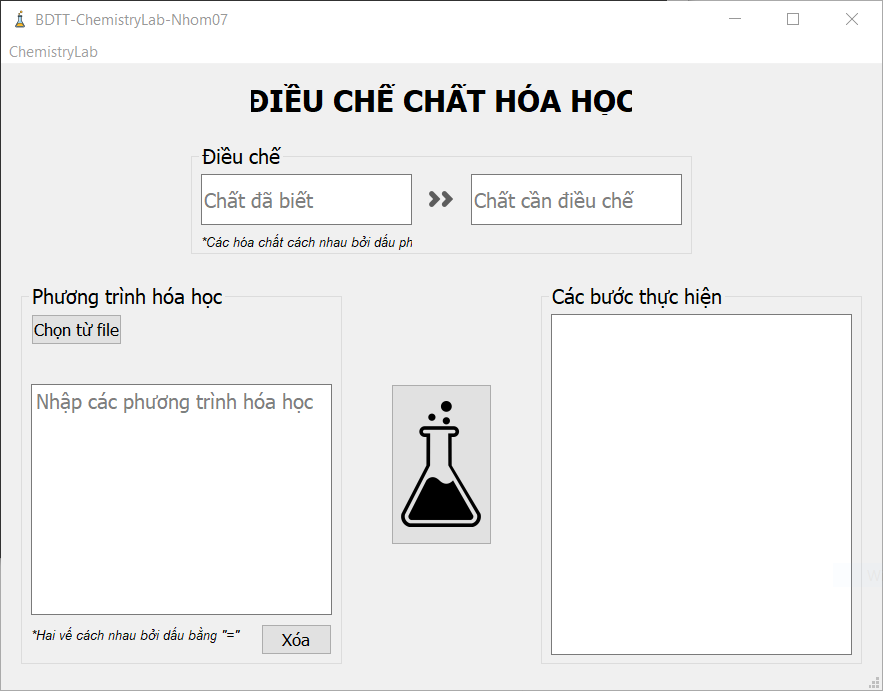
\includegraphics[width=.7\linewidth]{hdsd1}
		\caption{Màn hình giao diện}
		\label{screen}
	\end{figure}
	\begin{itemize}
		\item \textbf{Quy ước định dạng phương trình hóa học và hóa chất:} 
		\begin{itemize}
			\item Các chất hóa học như \texttt{Cl$_2$, H$_2$O, SO$_2$,...} sẽ được đưa vào dưới dạng \texttt{Cl\_2, H\_2O, SO\_2,...}
			\item Dấu mũi tên trong các phương trình hóa học sẽ được thay bởi dấu bằng "=". Ví dụ: \texttt{2Na+Cl$_2$ $\rightarrow$ 2NaCl} sẽ được đưa vào dưới dạng \texttt{2Na+Cl\_2 = 2NaCl}
		\end{itemize}
		\item \textbf{Điều chế:} Người dùng nhập các chất hóa học đã có (nguyên liệu điều chế) vào ô \textcolor{blue}{\texttt{Chất đã biết}} (bên trái), và nhập các chất hóa học cần điều chế vào ô \textcolor{blue}{\texttt{Chất cần điều chế}} (bên phải). 
		
		Trong quá trình nhập liệu, người dùng sử dụng \textbf{dấu phẩy (,)} để ngăn cách các hóa chất, lưu ý không sử dụng dấu cách (khoảng trắng).
		
		Ở ô \textcolor{blue}{\texttt{Chất đã biết}}, chương trình đã mặc định có hóa chất \texttt{O$_2$}, vì hóa chất này có sẵn trong không khí.
		
		\item \textbf{Phương trình hóa học:} Người dùng có thể đưa tri thức (các phương trình hóa học) vào chương trình bằng 2 cách
		\begin{itemize}
			\item Nhập trực tiếp: người dùng nhập các phương trình hóa học, theo đúng định dạng quy ước, vào ô trống. Các phương trình ngăn cách nhau bởi kí hiệu ngắt dòng (Enter).
			\item Nhập từ file: người dùng chọn \textcolor{blue}{\texttt{Chọn từ file}} và chọn tệp tin chứa các phương trình hóa học cần đưa vào, lưu ý rằng chỉ có thể chọn 1 tệp tin (định dạng txt). Lúc này các phương trình hóa học trong tệp tin sẽ được hiển thị ở ô trống phía dưới.
		\end{itemize}
		Người dùng có thể chọn \texttt{Xóa} để xóa tất cả các phương trình hóa học vừa nhập.
		\item Sau khi cung cấp đủ thông tin ở hai phần \textbf{Điều chế} và \textbf{Phương trình hóa học}, người dùng chọn nút "lọ hóa chất" để chương trình tiến hành điều chế, kết quả sẽ được hiển thị ở ô \textbf{Các bước thực hiện}.
	\end{itemize}
Dưới đây là các bước thực hiện để điều chế \texttt{H$_2$SO$_4$} từ \texttt{S} và \texttt{H$_2$O}:
	\begin{figure}[h]
		\centering \includegraphics[width=.7\linewidth]{vd}
		\caption{Ví dụ}
		\label{screen}
	\end{figure}

\end{document}